\documentclass[11pt,a4paper]{article}
% Shared styling for the WaveKitchen documentation PDFs.
\usepackage[T1]{fontenc}
\usepackage{lmodern}
\usepackage[utf8]{inputenc}
\usepackage[margin=2.2cm,headheight=14pt]{geometry}
\usepackage{amsmath,amssymb}
\usepackage{xcolor}
\usepackage{booktabs,longtable,tabularx,array}
\usepackage{enumitem}
\usepackage{fancyhdr}
\usepackage{titlesec}
\usepackage[most]{tcolorbox}
\usepackage{tikz}
\usetikzlibrary{arrows.meta,positioning,shapes.geometric,calc,fit}
\usepackage{microtype}
\usepackage[hidelinks]{hyperref}
\urlstyle{tt}

\definecolor{wkorange}{HTML}{E0661E}
\definecolor{wkteal}{HTML}{0E8A8A}
\definecolor{wkink}{HTML}{1F2937}
\definecolor{wkgrey}{HTML}{6B7280}
\definecolor{wkred}{HTML}{B91C1C}
\definecolor{wkgreen}{HTML}{15803D}
\definecolor{wkpaper}{HTML}{FFF8EF}

\hypersetup{colorlinks=true,linkcolor=wkteal,urlcolor=wkteal,citecolor=wkteal}

\titleformat{\section}{\Large\bfseries\color{wkorange}}{\thesection}{0.8em}{}
\titleformat{\subsection}{\large\bfseries\color{wkink}}{\thesubsection}{0.7em}{}
\titleformat{\subsubsection}{\normalsize\bfseries\color{wkteal}}{\thesubsubsection}{0.6em}{}

\setlist{itemsep=2pt,topsep=4pt}
\setlength{\parskip}{4pt}
\setlength{\parindent}{0pt}
% long unbreakable code names: stretch spaces rather than overflow the margin
\setlength{\emergencystretch}{3em}
\renewcommand{\arraystretch}{1.25}
% ragged-right paragraph column (no stretched inter-word spaces in narrow cells)
\newcolumntype{P}[1]{>{\raggedright\arraybackslash}p{#1}}

% file paths (break at slashes) and code identifiers (underscore-safe)
\newcommand{\file}[1]{\nolinkurl{#1}}
\DeclareRobustCommand{\fn}[1]{\texttt{\detokenize{#1}}}
% plain text for PDF bookmarks when these appear in headings
\pdfstringdefDisableCommands{\def\file#1{#1}\def\fn#1{\detokenize{#1}}}

\newtcolorbox{conceptbox}[1][]{colback=wkteal!6,colframe=wkteal,fonttitle=\bfseries,
  title={Signals \& Systems concept#1},breakable,left=6pt,right=6pt,top=4pt,bottom=4pt}
\newtcolorbox{impactbox}[1][]{colback=wkorange!6,colframe=wkorange,fonttitle=\bfseries,
  title={Why it is here \& its impact#1},breakable,left=6pt,right=6pt,top=4pt,bottom=4pt}
\newtcolorbox{filesbox}{colback=wkink!4,colframe=wkink!70,fonttitle=\bfseries,
  title={Files involved},breakable,left=6pt,right=6pt,top=4pt,bottom=4pt,before upper=\raggedright}
\newtcolorbox{flagbox}[1][]{colback=wkred!5,colframe=wkred,fonttitle=\bfseries,
  title={\(\blacktriangle\) Flag: low or no impact#1},breakable,left=6pt,right=6pt,top=4pt,bottom=4pt}
\newtcolorbox{mathbox}[1]{colback=white,colframe=wkteal!70,fonttitle=\bfseries,
  title={#1},breakable,left=6pt,right=6pt,top=4pt,bottom=4pt}
\newtcolorbox{notebox}{colback=wkpaper,colframe=wkgrey!60,breakable,left=6pt,right=6pt,top=4pt,bottom=4pt}

\pagestyle{fancy}
\fancyhf{}
\fancyfoot[C]{\small\color{wkgrey}\thepage}
\renewcommand{\headrulewidth}{0.3pt}

% station-flow diagram node styles
\tikzset{
  st/.style={draw=wkteal,fill=wkteal!8,rounded corners=3pt,minimum height=8mm,
    minimum width=21mm,align=center,font=\footnotesize},
  opt/.style={st,draw=wkorange,fill=wkorange!8,dashed},
  gate/.style={st,draw=wkink,fill=wkink!6},
  arr/.style={-Stealth,thick,color=wkink!70},
}

\fancyhead[L]{\small\color{wkgrey}WaveKitchen / WaveBakery}
\fancyhead[R]{\small\color{wkgrey}Detailed Gameplay Overview}

\begin{document}

% ---------------------------------------------------------------- title page
\begin{titlepage}
\centering
\vspace*{2.5cm}
{\color{wkorange}\rule{\linewidth}{1.2pt}}\\[0.6cm]
{\Huge\bfseries\color{wkink} WaveKitchen / WaveBakery}\\[0.35cm]
{\LARGE\color{wkteal} Detailed Gameplay Overview}\\[0.3cm]
{\large How the game plays, which files run each part, and how every station maps to Signals \& Linear Systems}\\[0.6cm]
{\color{wkorange}\rule{\linewidth}{1.2pt}}\\[1.6cm]

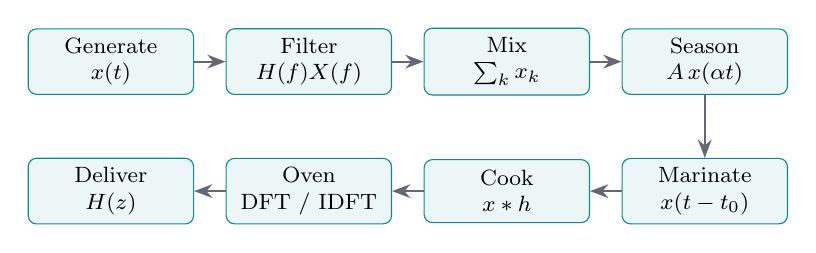
\begin{tikzpicture}[node distance=4mm]
\node[st] (a) {Generate\\$x(t)$};
\node[st,right=of a] (b) {Filter\\$H(f)X(f)$};
\node[st,right=of b] (c) {Mix\\$\sum_k x_k$};
\node[st,right=of c] (d) {Season\\$A\,x(\alpha t)$};
\node[st,below=8mm of d] (e) {Marinate\\$x(t-t_0)$};
\node[st,left=of e] (f) {Cook\\$x*h$};
\node[st,left=of f] (g) {Oven\\DFT / IDFT};
\node[st,left=of g] (h) {Deliver\\$H(z)$};
\draw[arr] (a)--(b); \draw[arr] (b)--(c); \draw[arr] (c)--(d); \draw[arr] (d)--(e);
\draw[arr] (e)--(f); \draw[arr] (f)--(g); \draw[arr] (g)--(h);
\end{tikzpicture}

\vfill
{\large CSE 220 --- Signals and Linear Systems project}\\[0.2cm]
{\color{wkgrey} Generated from the project source code (frontend \file{frontend/src}, backend \file{backend/app})}
\end{titlepage}

\tableofcontents
\newpage

% ====================================================================
\section{The game in one page}
% ====================================================================
WaveKitchen (the frontend calls itself \emph{WaveBakery}) is a cooking game in
which every culinary action is a signal-processing operation. Each
\textbf{ingredient is a signal}, each \textbf{kitchen station is a system}
that transforms the signal, and the \textbf{finished dish is the output} of the
whole chain. The player's goal is to make their dish match a hidden
\emph{reference dish}: the output of the same chain run with the recipe's ideal
parameters on clean ingredients.

\begin{center}
\begin{tabularx}{\linewidth}{@{}>{\bfseries}l X@{}}
\toprule
Kitchen idea & Signal-processing meaning \\
\midrule
Ingredient & A signal $x(t)$ (a periodic waveform, a parametric curve, or a recorded sound) \\
Dirty ingredient & Signal plus additive noise $x(t)+n(t)$ \\
Washing & Frequency-selective filtering (FFT $\rightarrow$ mask $\rightarrow$ IFFT) \\
Mixing bowl & Superposition $\sum_k x_k(t)$ (linearity) \\
Seasoning & Amplitude scaling $A\,x(t)$ and time scaling $x(\alpha t)$ \\
Marinating & Time shift (delay) $x(t-t_0)$ \\
Caramelizing & Amplitude modulation $x(t)\,[1+m\cos(2\pi f_c t)]$ \\
Chopping & Sampling / decimation and aliasing \\
Cooking appliance & An LTI system with impulse response $h[n]$; cooking is convolution $y=x*h$ \\
Precision Oven & Sampling theorem, DFT/FFT, frequency-domain equalisation, IDFT reconstruction \\
Delivery cart & Discrete-time system $H(z)$: poles, zeros, stability, frequency response \\
Tasting table & Similarity metrics between the player's dish and the reference dish \\
\bottomrule
\end{tabularx}
\end{center}

A run is \textbf{timed} (5:00 on Easy down to 1:00 on MasterChef), stations are
\textbf{unlocked in order}, and at the end the dish is \textbf{scored}, turned
into \textbf{stars and points}, and placed on a \textbf{leaderboard}.

% ====================================================================
\section{How the project is built}
% ====================================================================
\subsection{Two halves}
\begin{description}[style=nextline,leftmargin=0.6cm]
\item[Frontend (what the player sees and hears)] React 19 + TanStack Router/Start,
  built with Vite, written in TypeScript. It synthesises every ingredient signal
  mathematically, runs the whole per-station pipeline in the browser, draws every
  graph, plays every sound through the Web Audio API, and keeps the run state in
  \texttt{localStorage}. Folder: \file{frontend/src}.
\item[Backend (the authoritative judge)] FastAPI + SQLAlchemy + SQLite, with NumPy/SciPy
  for DSP. It stores chefs, sessions, attempts and the leaderboard. On submission it
  \emph{re-builds the dish from scratch} from the recorded parameters (it never trusts
  audio sent by the client) and scores it against the reference dish. Folder:
  \file{backend/app}.
\item[Runner] \file{run.py} starts both servers with one command (backend on port 8000,
  Vite on port 5173, which proxies \texttt{/api} to the backend).
\end{description}

\subsection{Most important files}
\begin{longtable}{@{}P{6.1cm}P{9.4cm}@{}}
\toprule
File & Role \\
\midrule
\endhead
\file{frontend/src/lib/signals.ts} & Every ingredient's mathematical signal (equations, parametric curves, the recorded chicken), and the mixing-bowl superposition curve. \\
\file{frontend/src/lib/pipeline.ts} & The per-station DSP pipeline: mixing, seasoning, marinating, convolution, the reference dish, curve carrying, stage storage and invalidation. \\
\file{frontend/src/lib/dsp.ts} & FFT, low-pass filtering, convolution, and the similarity metric used for the final score. \\
\file{frontend/src/lib/precision-oven-dsp.ts} & Sampling/aliasing analysis, radix-2 FFT/IFFT, oven equaliser, reconstruction and oven metrics. \\
\file{frontend/src/lib/z-system.ts} & Delivery-cart systems: poles, zeros, gain, difference equation, stability score. \\
\file{frontend/src/lib/cooking-audio.ts} & The four cooking impulse responses $h[n]$ (grill, fry, bake, boil). \\
\file{frontend/src/lib/audio.ts} & Turns a 401-sample signal into audible sound. \\
\file{frontend/src/lib/recipes.ts} & Recipe book, difficulty/timer, run session, progression, backend sync and submission. \\
\file{frontend/src/lib/leaderboard.ts} & The on-device leaderboard. \\
\file{frontend/src/lib/api.ts} & HTTP client for the backend. \\
\file{frontend/src/routes/*.tsx} & One file per screen/station (Section~\ref{sec:journey}). \\
\file{backend/app/dsp/core.py} & Backend DSP primitives: FFT, masks, filters, convolution, time operators, modulation, decimation. \\
\file{backend/app/dsp/instruments.py} & Backend ingredient synthesis (instrument-like voices). \\
\file{backend/app/dsp/contamination.py} & Seeded noise that makes ingredients ``dirty''. \\
\file{backend/app/dsp/systems.py} & Appliance impulse responses (comb, decay, resonator, moving average, differencer). \\
\file{backend/app/dsp/pipeline.py} & The canonical backend pipeline \fn{run_pipeline}. \\
\file{backend/app/dsp/metrics.py} & Prep (cleaning) score and dish score. \\
\file{backend/app/gameplay.py} & Judging, points, ranks, tier unlocks, System Delivery score. \\
\file{backend/app/routers/*.py} & HTTP endpoints: players, sessions, leaderboard, catalogue, direct DSP. \\
\file{backend/app/seed.py} & Ingredient, appliance and recipe catalogue (with targets). \\
\bottomrule
\end{longtable}

\subsection{A signal inside the frontend}
Every stage passes around a \fn{PipelineSignal} (defined in
\file{frontend/src/lib/pipeline.ts}): \textbf{401 samples} spanning a
\emph{normalised one-second window}. Frequencies inside the game are therefore
``game hertz'': cycles per window. A 4\,Hz ingredient shows 4 cycles on screen.
When a signal is played, \file{frontend/src/lib/audio.ts} repeats the window fast
enough that its fundamental becomes an audible pitch between 110 and 880\,Hz, so
what you hear has the same shape as what you see.

% ====================================================================
\section{The player's journey}\label{sec:journey}
% ====================================================================
\begin{center}
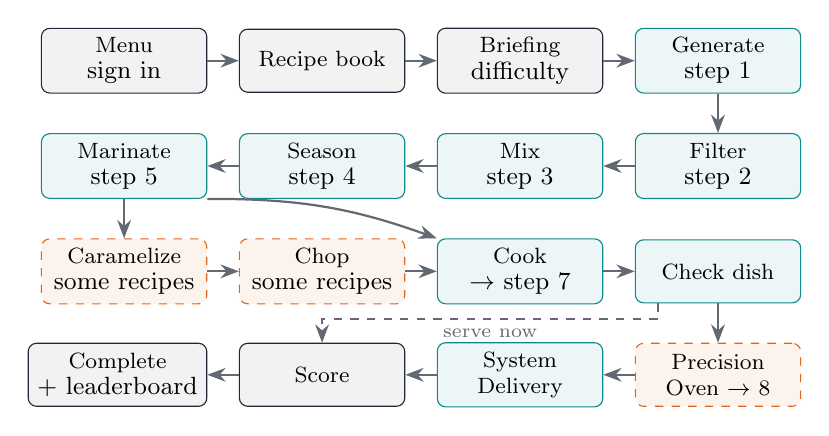
\begin{tikzpicture}[node distance=5mm and 4mm]
\node[gate] (menu) {Menu\\\small sign in};
\node[gate,right=of menu] (book) {Recipe book};
\node[gate,right=of book] (brief) {Briefing\\\small difficulty};
\node[st,right=of brief] (gen) {Generate\\\small step 1};
\node[st,below=of gen] (fil) {Filter\\\small step 2};
\node[st,left=of fil] (mix) {Mix\\\small step 3};
\node[st,left=of mix] (sea) {Season\\\small step 4};
\node[st,left=of sea] (mar) {Marinate\\\small step 5};
\node[opt,below=of mar] (car) {Caramelize\\\small some recipes};
\node[opt,right=of car] (chop) {Chop\\\small some recipes};
\node[st,right=of chop] (cook) {Cook\\\small $\rightarrow$ step 7};
\node[st,right=of cook] (chk) {Check dish};
\node[opt,below=of chk] (oven) {Precision\\Oven $\rightarrow$ 8};
\node[st,left=of oven] (sys) {System\\Delivery};
\node[gate,left=of sys] (score) {Score};
\node[gate,left=of score] (done) {Complete\\\small + leaderboard};
\draw[arr] (menu)--(book); \draw[arr] (book)--(brief); \draw[arr] (brief)--(gen);
\draw[arr] (gen)--(fil); \draw[arr] (fil)--(mix); \draw[arr] (mix)--(sea); \draw[arr] (sea)--(mar);
\draw[arr] (mar)--(car); \draw[arr] (car)--(chop); \draw[arr] (chop)--(cook);
\draw[arr] (mar.south east) to[bend left=10] (cook.north west);
\draw[arr] (cook)--(chk); \draw[arr] (chk)--(oven); \draw[arr] (oven)--(sys); \draw[arr] (sys)--(score);
\draw[arr,dashed] ([xshift=3mm]chk.south west) -- ++(0,-2mm) -| node[pos=0.25,below,font=\scriptsize]{serve now} (score.north);
\draw[arr] (score)--(done);
\end{tikzpicture}
\end{center}
Dashed orange boxes are optional or recipe-specific. Numbers are the progression
levels stored in \texttt{localStorage} (\fn{wavebakery_progress_<recipe>}): a
station stays locked (``Station Locked'' screen) until the previous level is
reached.

\subsection{Screens around the kitchen}
\begin{longtable}{@{}P{3.1cm}P{5.3cm}P{7.0cm}@{}}
\toprule
Screen & File & What happens \\
\midrule
\endhead
Landing / Menu & \file{routes/index.tsx}, \file{routes/menu.tsx} & Entry point; opens the chef sign-in (\file{components/game/ChefAuthModal.tsx}), leaderboard, settings, how-to-play and the Signal Playground. \\
Chef sign-in & \file{components/game/ChefAuthModal.tsx} & Register or sign in with name + password; the backend returns a token that identifies the chef on every later request. \\
Recipe book & \file{routes/recipe-book.tsx} & Choose one of 10 recipes; shows tier, difficulty and best score. \\
Briefing & \file{routes/briefing.tsx} & Shows the recipe's ingredients, and lets the player choose difficulty (timer). Starting calls \fn{startRecipeRun}, which resets progress, creates the run session and (if signed in) a backend game session. \\
Kitchen map / hub & \file{routes/kitchen.tsx}, \file{routes/kitchen-hub.tsx} & Station map and navigation hub. \\
Pantry & \file{routes/pantry.tsx} & Browse every ingredient and inspect its equation, waveform and spectrum (\file{components/game/IngredientSignalModal.tsx}). \\
Settings / How to play & \file{routes/settings.tsx}, \file{routes/how-to-play.tsx} & Theme, chef name, logout; the tutorial. \\
Leaderboard & \file{routes/leaderboard.tsx} & Server rankings per recipe/difficulty, global chef ranking, kitchen analytics, plus the on-device list when offline. \\
\bottomrule
\end{longtable}

\subsection{Difficulty and the timer}
\begin{center}
\begin{tabular}{lccl}
\toprule
Difficulty & Time & Score multiplier & Source \\
\midrule
Easy & 5:00 & $\times0.8$ & \fn{DIFFICULTY_CONFIGS} in \file{lib/recipes.ts}, \\
Medium & 3:30 & $\times1.0$ & multipliers in \file{routes/score.tsx} \\
Hard & 2:00 & $\times1.25$ & \\
MasterChef & 1:00 & $\times1.5$ & \\
\bottomrule
\end{tabular}
\end{center}
The timer (\fn{useRecipeTimer}) counts down from the run's start. When it hits zero
an expiry dialog (\file{components/game/RecipeTimer.tsx}) blocks the run and offers a
retry; no completion score is awarded for an expired run. Time left at the end
becomes a bonus (Section~\ref{sec:score}).

% ====================================================================
\section{Station by station}
% ====================================================================
Each station below lists what the player does, the files that implement it, the
Signals \& Systems concept it teaches, and why it exists and what it changes in the
final result.

% --------------------------------------------------------------------
\subsection{Pantry and Generate Signal --- ingredients are signals}
\textbf{What the player does.} Picks ingredients for the recipe, sees each
ingredient's equation, waveform and spectrum, and listens to it. Finishing
unlocks Filtering (or Mixing directly if nothing needs washing).

\begin{filesbox}
\file{frontend/src/routes/generate.tsx} (station), \file{frontend/src/routes/pantry.tsx},
\file{frontend/src/lib/signals.ts} (all ingredient models), \fn{getRecipeIngredientSamples}
in \file{frontend/src/lib/pipeline.ts}, \file{frontend/src/lib/chicken-audio.ts} and
\file{frontend/src/lib/chicken-samples.ts} (recorded chicken), \file{frontend/src/lib/audio.ts}.
\end{filesbox}

The ingredients form a small catalogue of textbook signal families:
\begin{longtable}{@{}P{2.3cm}P{2.4cm}P{11.1cm}@{}}
\toprule
Ingredient & Family & Model (from \file{lib/signals.ts}) \\
\midrule
\endhead
Cheese & triangle & $x(t)=A\tfrac{2}{\pi}\arcsin(\sin(2\pi ft+\phi))$ --- odd harmonics, $1/n^2$ roll-off \\
Sugar & square & $x(t)=A\,\mathrm{sgn}(\sin(2\pi ft+\phi))$ --- odd harmonics, $1/n$ roll-off \\
Salt & square & same as sugar with small amplitude $A_s=0.4$ \\
Bread & superposition & $y(t)=0.8\sin(6\pi t)+0.6\sin(18\pi t)$ (3\,Hz + 9\,Hz) \\
Milk & sum of sines & $y=1.4\sin(0.7x)+0.6\sin(1.3x)+0.3\sin(2.1x+0.8)$ (non-harmonic) \\
Flour & ``flame'' & $\mathrm{sq}(t)-\mathrm{sq}(2t)\cos(2\pi t)$ (product of signals) \\
Bun & dome & $5(0.5+0.5\cos 0.3x)^{0.25}+0.03\cos 9x$ \\
Butter & trapezoid & $\max(0,\,1.2-1.2\max(|\mathrm{mod}(x+9,14)-9|-4,0))$ \\
Carrot & taper & $5-(1+\cos 0.5x)^4$ \\
Cucumber & saturated & $6\tanh(4\cos x)$ --- a soft-clipped cosine \\
Beef patty & parametric & $x=2.5\cos t+5\lfloor t/2\pi\rfloor,\ y=0.7\sin t$ \\
Lettuce & parametric & $x=t,\ y=2.2\cos t+0.45\cos 7.5t$ \\
Noodles & parametric & $x=t+3\sin t,\ y=5\cos t$ (trochoid loops) \\
Tomato & parametric & $x=(2+0.2\sin3t)\cos t,\ y=-(1.5+0.2\sin t)\sin t$ \\
Onion & parametric & $x=(0.1+0.08t)\cos3t,\ y=(0.1+0.08t)\sin 3t$ (spiral) \\
Sauce & parametric & $x=(3+2\sin5t)\cos t,\ y=(2+\sin5t)\sin t$ \\
Egg & parametric & $x=(1.5+0.5\sin t)\cos t,\ y=-(2+0.2\sin t)\sin t$ \\
Chicken & recorded & $s(t)=$ PCM samples of \file{public/sounds/chicken.wav} (44.1\,kHz) \\
\bottomrule
\end{longtable}

A \emph{parametric} ingredient is a 2-D curve $(x(t),y(t))$. For sound and for the
1-D pipeline the game uses its vertical component $y(t)$ as the time signal; for the
mixing-bowl picture it keeps the full curve.

\begin{conceptbox}
Continuous-time signal models and their classification: periodic vs aperiodic,
sinusoids, square/triangle waves and their Fourier-series harmonic content,
superposition of sinusoids, nonlinear shaping (saturation, clipping), parametric
curves, and a real sampled recording (discrete-time signal at 44.1\,kHz).
\end{conceptbox}
\begin{impactbox}
Every later station operates on these signals, so this is the input to the whole
system. Choosing ingredients decides what goes into the bowl; a wrong or missing
ingredient changes the mix and lowers the Mixing accuracy and the final similarity.
Different families were chosen so the player can \emph{see} why a square wave has
a richer spectrum than a sine and why filtering affects them differently.
\end{impactbox}

% --------------------------------------------------------------------
\subsection{Filtering Lab --- washing is filtering}
\textbf{What the player does.} Each \emph{washable} ingredient arrives with noise.
The player drags a \textbf{cutoff frequency} slider over the spectrum, applies the
filter and must reach a cleanliness of at least 85\,\% before moving on.

\begin{filesbox}
\file{frontend/src/routes/filtering.tsx}; \fn{applyLowPassFilter}, \fn{fft} in
\file{frontend/src/lib/dsp.ts}; backend \fn{apply_filters} / \fn{accept_ingredient}
in \file{backend/app/routers/sessions.py}; \fn{dirty_signal}, \fn{filtered_signal}
in \file{backend/app/gameplay.py}; \file{backend/app/dsp/contamination.py};
\fn{apply_filter_chain} in \file{backend/app/dsp/pipeline.py}; \fn{prep_quality} in
\file{backend/app/dsp/metrics.py}.
\end{filesbox}

When a backend session exists, the Filtering Lab shows the \emph{server's} real
dirty and clean signal for that ingredient, sends the chosen cutoff to the server
(\fn{filterIngredient}), and displays the server's filtered result and cleaning
score. Offline, a local approximation is used. The filtered samples are saved and
become the ingredient's input to Mixing.

\begin{conceptbox}
Additive noise, the Fourier transform (FFT), the frequency domain, ideal vs
practical low-pass filters (a raised-cosine transition band), filtering as
multiplication in frequency $Y(f)=H(f)X(f)$, and the trade-off between removing
noise and keeping the signal's own frequencies (cutting too low distorts the
ingredient).
\end{conceptbox}
\begin{impactbox}
It is the first place the player must reason in the frequency domain. The server's
cleaning (``prep'') score is 28\,\% of the authoritative dish score and is reported
as the Filtering sub-score; the local filtering accuracy is one of the stage
averages in the offline score. Over-filtering is detected and named in the feedback
(``you cut real ingredient frequencies'').
\end{impactbox}

% --------------------------------------------------------------------
\subsection{Mixing Lab --- the bowl is superposition}
\textbf{What the player does.} Drags ingredients from the tray into the bowl and
presses \emph{Mix}. The oscilloscope shows each ingredient and the combined signal.

\begin{filesbox}
\file{frontend/src/routes/mixing.tsx}; \fn{computeMixedSignal},
\fn{withMixCurve}, \fn{getMixingIngredientSamples} in \file{frontend/src/lib/pipeline.ts};
\fn{computeSuperpositionCurve}, \fn{computeSuperpositionPath} in
\file{frontend/src/lib/signals.ts}; backend \fn{bowl_signals}, \fn{compute_stages} in
\file{backend/app/gameplay.py} and \fn{stage_mix} in \file{backend/app/dsp/pipeline.py}.
\end{filesbox}

For ordinary ingredients the mix is the sample-by-sample sum. When a parametric
ingredient is present the bowl draws the \emph{2-D geometric} superposition
$(\sum_k x_k(t),\ \sum_k y_k(t))$, which is why curves such as noodles make loops.
That curve is carried as a visual track through every later station. The bowl
contents are sent to the server, which mixes exactly those ingredients.

\begin{conceptbox}
Linearity and the superposition principle; normalisation of a sum
($1/\sqrt{K}$) to keep amplitude comparable; the difference between adding signals
in time and adding curves in the plane.
\end{conceptbox}
\begin{impactbox}
Mixing accuracy is the fraction of recipe ingredients correctly placed. On the
server, missing or extra ingredients change the mixed signal and therefore the
Mixing sub-score and every stage after it.
\end{impactbox}

% --------------------------------------------------------------------
\subsection{Seasoning Lab --- amplitude and time scaling}
\textbf{What the player does.} Sets \emph{Signal strength} (amplitude $A$) and
\emph{Frequency character} ($\alpha$) and watches the player curve approach the
dashed target curve. Accuracy $\geq 85\,\%$ completes the station.

\begin{filesbox}
\file{frontend/src/routes/transform.tsx}; \fn{computeSeasonedSignal},
\fn{timeScaleSamples}, \fn{transformCurve} in \file{frontend/src/lib/pipeline.ts};
backend \fn{stage_season} and \fn{stage_blend} (\fn{time_scale}) in
\file{backend/app/dsp/pipeline.py} and \file{backend/app/dsp/core.py}.
\end{filesbox}
\begin{conceptbox}
Amplitude scaling $y(t)=A\,x(t)$ and time scaling $y(t)=x(\alpha t)$: $\alpha>1$
compresses the signal (higher frequencies, more cycles), $\alpha<1$ expands it.
Time scaling scales the spectrum: $x(\alpha t)\leftrightarrow\frac{1}{|\alpha|}X(f/\alpha)$.
\end{conceptbox}
\begin{impactbox}
The dials are synced to the server (as \texttt{seasoning} and \texttt{blend}); a
wrong gain or rate changes the reference comparison and triggers named feedback
(``over-seasoned'', ``over-blended''). The seasoning accuracy is a stage average and
half of the ``Transformation'' score.
\end{impactbox}

% --------------------------------------------------------------------
\subsection{Marinating Lab --- time shift}
\textbf{What the player does.} Chooses a marinating time; the waveform is delayed
(a flat lead-in, then the signal) and must match the target timing.

\begin{filesbox}
\file{frontend/src/routes/marinate.tsx}; \fn{computeMarinatedSignal},
\fn{delayCurve} in \file{frontend/src/lib/pipeline.ts}; backend \fn{stage_marinate}
and \fn{time_shift} (fractional delays via a linear phase ramp) in
\file{backend/app/dsp/pipeline.py} and \file{backend/app/dsp/core.py}.
\end{filesbox}
\begin{conceptbox}
Time shifting $y(t)=x(t-t_0)$; causality and zero padding; the shift theorem
$x(t-t_0)\leftrightarrow X(f)e^{-j2\pi f t_0}$, which the backend uses to delay by
non-integer numbers of samples.
\end{conceptbox}
\begin{impactbox}
The time is synced to the server as \texttt{marinate} (seconds). It completes the
Transformation score together with seasoning, and the server names mistakes
(``marinated too long --- excess time shift'').
\end{impactbox}

% --------------------------------------------------------------------
\subsection{Caramelize Lab --- amplitude modulation (Crème Brûlée, Feast)}
\textbf{What the player does.} Sets a carrier frequency $f_c$ and modulation depth
$m$ and listens to the ``caramelized'' signal.

\begin{filesbox}
\file{frontend/src/routes/caramelize.tsx}; backend \fn{stage_caramelize} /
\fn{am_modulate} in \file{backend/app/dsp/pipeline.py} and \file{backend/app/dsp/core.py};
targets in \file{backend/app/seed.py}.
\end{filesbox}
\begin{conceptbox}
Amplitude modulation $y(t)=x(t)[1+m\cos(2\pi f_c t)]$: the spectrum gains
sidebands at $f\pm f_c$; the depth $m$ sets their height.
\end{conceptbox}
\begin{impactbox}
Carrier and depth are sent to the server, whose pipeline modulates the dish before
cooking; the recipe's targets make the reference dish modulated too. The station
also has its own accuracy, averaged into the local score for recipes that need it.
\end{impactbox}

% --------------------------------------------------------------------
\subsection{Chop Lab --- sampling, decimation and aliasing (Salad, Feast)}
\textbf{What the player does.} Chooses a decimation factor $M$ and whether to use
an anti-aliasing filter.

\begin{filesbox}
\file{frontend/src/routes/chop.tsx}; backend \fn{stage_chop} / \fn{decimate} in
\file{backend/app/dsp/pipeline.py} and \file{backend/app/dsp/core.py}.
\end{filesbox}
\begin{conceptbox}
Down-sampling by $M$ (keep every $M$-th sample, zero-order hold back), the new
Nyquist frequency $f_s/(2M)$, aliasing when content exceeds it, and the
anti-aliasing low-pass filter that prevents it.
\end{conceptbox}
\begin{impactbox}
Factor and filter choice are sent to the server, which decimates for real before
cooking; skipping the anti-alias filter is diagnosed (``Aliasing! You decimated
without the anti-alias filter'').
\end{impactbox}

% --------------------------------------------------------------------
\subsection{Cooking Lab --- convolution with an appliance}
\textbf{What the player does.} Picks a cooking method (grill, fry, bake, boil ---
each is an impulse response) and slides the impulse across the signal to set the
convolution depth. The panels show input $x$, impulse response $h$, output $x*h$
and the target.

\begin{filesbox}
\file{frontend/src/routes/cooking.tsx}; \fn{computeConvolvedSignal} in
\file{frontend/src/lib/pipeline.ts}; kernels in \file{frontend/src/lib/cooking-audio.ts};
backend \fn{stage_cook}, \fn{apply_system}, \fn{cascade} and the appliance impulse
responses in \file{backend/app/dsp/systems.py}.
\end{filesbox}
\begin{conceptbox}
Linear time-invariant (LTI) systems are fully described by the impulse response;
the output is the convolution $y[n]=\sum_k x[k]\,h[n-k]$. Different $h$ give
different characters: a comb of echoes (grill), a bright decaying burst (fry), a
smooth long tail / low-pass (bake), a damped resonator (boil). A cascade of LTI
systems is one LTI system with $h=h_1*h_2*\cdots$.
\end{conceptbox}
\begin{impactbox}
The chosen appliance is the heart of the dish. The server's Cooking sub-score now
isolates this choice: it compares the player's pre-cooking signal through the
recipe's appliances against the same signal through the player's appliances, so the
right appliance scores 100 even if earlier stages were imperfect.
\end{impactbox}

% --------------------------------------------------------------------
\subsection{Check Dish}
\textbf{What the player does.} Inspects and listens to the cooked dish, then either
serves it immediately or takes it to the Precision Oven
(\file{components/beamforming/ServeChoiceModal.tsx}).
\begin{filesbox}\file{frontend/src/routes/check-dish.tsx}, \file{frontend/src/components/game/WaveformDisplay.tsx}.\end{filesbox}
\begin{impactbox}
No computation of its own: it is a checkpoint that lets the player hear the result
of convolution before the optional finishing stations.
\end{impactbox}

% --------------------------------------------------------------------
\subsection{Precision Oven --- sampling theorem and the DFT}
\textbf{What the player does.} Five steps:
\begin{enumerate}
\item \textbf{Sampling}: pick a sampling rate $f_s$ and watch the reconstruction; below
  $2f_{\max}$ the dish aliases.
\item \textbf{Unlock}: type the minimum safe rate; it must satisfy $f_s\geq 2f_{\max}$ and
  be at most 64\,Hz.
\item \textbf{FFT lab}: see the dish's spectrum next to the target's and tune three
  bands (Base Warmth 0--6\,Hz, Crumb 6--16\,Hz, Top Crisp 16--32\,Hz), a browning cutoff
  and a charred-notch filter.
\item \textbf{IFFT}: rebuild the dish from the edited spectrum and listen.
\item \textbf{Plate}: save the result as the delivered dish.
\end{enumerate}
\begin{filesbox}
\file{frontend/src/routes/beam-delivery.tsx} (the Precision Oven screen; the file name
is historical), \file{frontend/src/lib/precision-oven-dsp.ts}, \fn{computeSignalSimilarity}
in \file{frontend/src/lib/dsp.ts}.
\end{filesbox}
\begin{conceptbox}
The Nyquist--Shannon sampling theorem, aliasing and frequency folding, the DFT and
its frequency axis $f_k=k f_s/N$, zero padding, the radix-2 Cooley--Tukey FFT,
frequency-domain filtering, Hermitian symmetry of real signals, the inverse DFT, and
band-limited (sinc/Dirichlet) reconstruction.
\end{conceptbox}
\begin{impactbox}
The oven score (spectrum match 40\,\%, waveform fidelity 50\,\%, sampling efficiency
10\,\%) becomes the Precision Oven Finishing accuracy, which counts for 10\,\% of the
dish score on both the score screen and the server.
\end{impactbox}

% --------------------------------------------------------------------
\subsection{System Delivery --- the z-plane}
\textbf{What the player does.} Chooses the cart's ``suspension'' (a 1st-order
low-pass, a 2nd-order resonator, a moving average or a notch), drags the pole on
the z-plane (radius $r$, angle $\omega_0$) and picks the sensor sampling rate. The
screen shows poles/zeros, $|H(e^{j\omega})|$, phase, the dish spectrum before and
after the cart, and an impulse-response animation; ``Listen equalized dish'' plays
the dish filtered by the cart.
\begin{filesbox}
\file{frontend/src/routes/system-delivery.tsx}, \file{frontend/src/components/system/SystemResponsePlotter.tsx},
\file{frontend/src/lib/z-system.ts}; backend \fn{system_score_for} in \file{backend/app/gameplay.py}.
\end{filesbox}
\begin{conceptbox}
The z-transform, transfer functions $H(z)=g\,\prod(z-z_i)/\prod(z-p_j)$, difference
equations, poles and zeros, BIBO stability (all poles inside $|z|=1$), frequency
response on the unit circle, FIR (moving average) vs IIR (resonator, low-pass) systems.
\end{conceptbox}
\begin{impactbox}
A stable, alias-free cart scores 100 (unstable 15, and $\times0.6$ below a 4\,kHz
sensor). The server recomputes this from the settings and counts it for 5\,\% of
the dish score.
\end{impactbox}

% --------------------------------------------------------------------
\subsection{Score, Complete and the leaderboard}\label{sec:score}
\textbf{What the player sees.} The score screen compares the player's dish with the
target (waveforms and a similarity percentage), shows the stage breakdown, stars,
Chef Fourier's feedback and a customer critique, and the total points. The
Complete page repeats the score and stars; the leaderboard ranks the run.
\begin{filesbox}
\file{frontend/src/routes/score.tsx}, \file{frontend/src/routes/complete.tsx},
\file{frontend/src/lib/critiques.ts}, \file{frontend/src/lib/leaderboard.ts},
\file{frontend/src/routes/leaderboard.tsx}; backend \fn{submit} in
\file{backend/app/routers/sessions.py}, \fn{judge}, \fn{award}, \fn{maybe_unlock} in
\file{backend/app/gameplay.py}, \file{backend/app/dsp/metrics.py},
\file{backend/app/routers/leaderboard.py}.
\end{filesbox}
How it works in short:
\begin{enumerate}
\item The latest parameters are synced, then the run is submitted once.
\item The server rebuilds the player's dish and the reference dish, computes a
  0--100 score and stars (92/80/66/50/32 for 5--1 stars), points and possible tier
  unlocks. Offline, the browser computes a 0--100 score with the same weighting.
\item Total points on screen $=$ score $\times10\times$ difficulty multiplier $+$ a
  time bonus (2 per second left, at most 300, also $\times$ difficulty).
\item The run is saved to the on-device leaderboard; the server leaderboard keeps
  each chef's best dish per recipe (filterable by difficulty).
\end{enumerate}
\begin{conceptbox}
Signal similarity measures: normalised cross-correlation, (normalised) mean-square
error and SNR in dB, and spectral similarity (cosine similarity of dB magnitude
spectra).
\end{conceptbox}
\begin{impactbox}
This is where every earlier decision becomes a number; the full formulas are in
the \emph{Detailed Architecture} document.
\end{impactbox}

% --------------------------------------------------------------------
\subsection{Signal Playground (Labs) --- a sandbox}
\file{frontend/src/routes/labs.tsx} offers free-play sandboxes: generator, filter,
mixer, seasoning, marinating, convolution and a \textbf{beamforming lab} (phased
speaker array, steering and windowing, \file{frontend/src/lib/beamforming.ts} and
\file{frontend/src/components/beamforming/*}). Nothing here affects a recipe run or
the score; it exists for exploration and teaching.

% ====================================================================
\section{The recipes}
% ====================================================================
{\small\setlength{\tabcolsep}{4pt}
\begin{longtable}{@{}P{2.0cm}P{0.6cm}P{4.8cm}P{1.6cm}P{1.2cm}P{1.0cm}P{3.0cm}@{}}
\toprule
Recipe & Tier & Ingredients & Season $A,\alpha$ & Marin. & Cook & Extra \\
\midrule
\endhead
Burger & 1 & Bun, Beef Patty, Cheese, Lettuce, Tomato, Salt & 1.5, 0.8 & 1.25 & grill & --- \\
Sandwich & 1 & Bread, Chicken, Cheese, Lettuce, Tomato, Salt, Sauce & 1.2, 1.1 & 0.85 & grill & --- \\
Golden Toast & 1 & Cheese & 1.0, 1.0 & 1.0 & bake & --- \\
Cake & 2 & Flour, Egg, Butter, Sugar, Milk & 1.8, 0.6 & 1.5 & bake & --- \\
Noodles & 2 & Noodles, Egg, Chicken, Onion, Salt & 1.3, 1.2 & 1.75 & boil & --- \\
Velvet Soup & 2 & Onion, Salt, Butter & 0.65, 0.7 & 1.05 & boil & --- \\
Crisp Salad & 2 & Lettuce, Tomato, Cucumber & 0.9, 1.0 & 1.02 & grill & Chop $M=3$ \\
Chicken Fry & 3 & Chicken, Flour, Egg, Salt, Butter & 2.0, 1.4 & 1.4 & fry & --- \\
Crème Brûlée & 3 & Egg, Sugar, Milk, Butter & 0.75, 0.85 & 1.16 & bake & AM 180, 0.55 \\
Grand Feast & 4 & Beef Patty, Cheese, Tomato, Lettuce, Bun & 0.95, 1.25 & 1.2 & grill & Chop $M=2$; AM 240, 0.4 \\
\bottomrule
\end{longtable}}
Targets live in \file{frontend/src/lib/recipes.ts} and, for the server,
\file{backend/app/seed.py}; the two are kept identical.

\subsection{Chef progression}
\begin{itemize}
\item \textbf{Points}: a served dish earns $\lfloor\text{score}\times\text{tier}\times1.5\rceil$
  points, but only if it beats the chef's previous best on that recipe, and only on an
  unlocked tier (locked-tier runs are ranked but earn nothing).
\item \textbf{Ranks} (by total points): Dishwasher 0, Prep Cook 250, Line Cook 600,
  Sous Chef 1100, Head Chef 1800, Signal Master 2600.
\item \textbf{Tiers}: clearing 2 recipes of the current tier with a score $\geq 60$
  unlocks the next tier.
\end{itemize}

% ====================================================================
\section{Alignment with Signals \& Linear Systems}
% ====================================================================
\begin{longtable}{@{}P{3.4cm}P{2.9cm}P{4.2cm}P{4.3cm}@{}}
\toprule
Concept & Where & Why it was added & Impact on the game \\
\midrule
\endhead
Signal classification, periodic signals, harmonics & Pantry, Generate & Ingredients must look and sound different for reasons the player can explain & Defines every input; wrong choice lowers Mixing \\
Fourier transform / spectrum & Filtering, Oven, Delivery & Noise is easier to see and remove in frequency & Drives the cleaning score (28\,\% server weight) \\
Filtering ($H(f)X(f)$) & Filtering & Washing = removing the noise band without cutting the ingredient & Prep score, over/under-filter feedback \\
Linearity / superposition & Mixing & A bowl is literally a sum & Mixing accuracy and server mix \\
Amplitude and time scaling & Seasoning & Two dials that change height and rate & Transformation score, server params \\
Time shift & Marinating & Delay is the simplest system & Transformation score, server params \\
Amplitude modulation & Caramelize & Sidebands as ``browning'' & Server pipeline (2 recipes) \\
Sampling, decimation, aliasing & Chop, Oven & Coarse chopping loses detail; Nyquist & Server pipeline (2 recipes); oven score \\
LTI systems, impulse response, convolution & Cooking & Each appliance is a system $h$ & Central to the dish; Cooking score \\
DFT/FFT, IDFT, zero padding, reconstruction & Precision Oven & Finishing in the frequency domain & 10\,\% of dish score \\
z-transform, poles/zeros, stability & System Delivery & A stable cart delivers the dish & 5\,\% of dish score \\
Correlation, MSE/SNR, spectral similarity & Score & Objective comparison with the target & The final score, stars, leaderboard \\
\bottomrule
\end{longtable}

% ====================================================================
\section{Parts with little or no impact (flagged)}\label{sec:flags}
% ====================================================================
While mapping the project, the following parts were found to be unrelated to the
Signals \& Systems content or to have no effect on the game's result.

\begin{flagbox}
\begin{enumerate}[leftmargin=*]
\item \textbf{Beamforming (Signal Playground only).} \file{frontend/src/lib/beamforming.ts},
  \file{frontend/src/components/beamforming/BeamformingVisualizer.tsx},
  \file{BeamPatternGraph.tsx}, \file{PhaseControls.tsx}, \file{SpeakerArray.tsx} are only
  used by the sandbox in \file{routes/labs.tsx}. \file{BeamTarget.tsx} is not used anywhere.
  Array processing is outside the core Signals \& Linear Systems syllabus and has no
  effect on any score.
\item \textbf{Backend phased-array endpoint} \fn{POST /api/sessions/\{id\}/beam-delivery}
  and \file{backend/app/dsp/beamforming.py}: never called by the frontend.
\item \textbf{Backend ``direct DSP'' endpoints} (\fn{/api/dsp/generate}, \fn{filter},
  \fn{mix}, \fn{transform}, \fn{convolve}, \fn{beamforming}, \fn{critique}) and their
  client methods in \file{lib/api.ts}: never called by the game.
\item \textbf{Unused client methods} in \file{lib/api.ts}: \fn{getConvolution},
  \fn{getHealth}, \fn{getPlayerHistory}, \fn{getRecipes}, \fn{getRecipe},
  \fn{getIngredients}, \fn{getAppliances}, \fn{loginPlayer}, \fn{registerPlayer}.
\item \textbf{Unreachable noise types}: \fn{corrupt} in \file{backend/app/dsp/contamination.py}
  only ever picks white, hiss or burst noise; its pink, hum and tone branches never run.
\item \textbf{WAV impulse-response loader} \fn{loadCookingImpulseAudio} in
  \file{frontend/src/lib/cooking-audio.ts}: never called; cooking always uses the static
  kernels.
\item \textbf{Sensor sampling-rate toggle} on System Delivery: it changes the score
  factor and colours, but the plotted spectrum does not change with it.
\item \textbf{Check Dish}: a checkpoint with no computation or score of its own.
\item \textbf{Chop Lab aliasing is simulated in the browser}: when anti-aliasing is off it
  adds a synthetic tone rather than genuinely folding frequencies (the server's
  \fn{decimate} does real aliasing).
\item \textbf{Hardcoded station targets}: the Caramelize and Chop pages score the player
  against fixed targets (180\,Hz / 0.55 and factor 3) instead of the recipe's own
  (\emph{Grand Feast} uses 240\,Hz / 0.4 and factor 2), so on the Feast the on-screen
  accuracy disagrees with the server.
\item \textbf{Two different ingredient models}: the server synthesises ingredients as
  instrument-like audio (\file{backend/app/dsp/instruments.py}) at 22\,050\,Hz, while the
  browser uses the mathematical models above. The server score is therefore computed on
  a different (but parameter-equivalent) dish than the one drawn on screen; only the
  Filtering Lab shows the server's own signals.
\item \textbf{Chop and Caramelize outputs are not drawn into later stations}: their
  signals are sent to the server and scored, but the Cooking Lab still draws the
  marinated signal as its input.
\end{enumerate}
\end{flagbox}

% ====================================================================
\section{Glossary}
% ====================================================================
\begin{description}[leftmargin=3.2cm,style=sameline]
\item[Game hertz] Cycles per normalised one-second window of 401 samples.
\item[Reference dish] The pipeline output for clean ingredients with the recipe's exact parameters.
\item[Stage accuracy] A 0--100 value each station records on the run session.
\item[Prep score] The server's cleaning score for a filtered ingredient.
\item[Session] The server's record of one run (seed, parameters, status).
\item[Attempt] A served dish on the server; the leaderboard's source.
\end{description}

\end{document}
